\documentclass[10pt]{beamer}

\usetheme{metropolis}
\usepackage{appendixnumberbeamer}

\usepackage{outlines}

\title{Extending Distributed Functionality in Phylanx}
\subtitle{Scientific Computing Around Louisiana}
\author{Maxwell Reeser}
\date{February 8, 2020}
\institute{Division of Computer Science and Engineering \\ School of Electrical Engineering and Computer Science \\ Louisiana State University}
\titlegraphic{
\includegraphics[height=10mm]{logos/stellar_4x1.pdf}}
\titlegraphic{
	\begin{tikzpicture}[overlay, remember picture]
	\node[at=(current page.south east), anchor=south east] {%
		
\includegraphics[width=.25\textwidth]{logos/stellar_4x1.pdf} 
	};
	\node[at=(current page.south west), anchor=south west] {%
		
\includegraphics[width=.50\textwidth]{logos/cct_logo.pdf} 
	};
	\end{tikzpicture}
}


\begin{document}
\setbeamercolor{background canvas}{bg=white}
\maketitle

%\begin{frame}{Outline}
%  \setbeamertemplate{section in toc}[sections]
%  \tableofcontents[hideallsubsections]
%\end{frame}
\begin{frame}{Outline}
	\setbeamertemplate{section in toc}[sections]
	\tableofcontents[hideallsubsections]
\end{frame}

\section{Introduction to Phylanx}

\begin{frame}{Phylanx: An Asynchronous Distributed C++ Array Processing Toolkit}
	\begin{outline}
		\1 Write Python code, run it in distributed
		\1 Targeting machine learning mainly
			\2 Focus on linear algebra
		\1 Heavy use of HPX			
			\2 Standard's compliant distributed C++ runtime
			\2 Product of Stellar Group
		\1 Blaze data structures
			\2 Parallelism already implemented
	\end{outline}
\end{frame}



\begin{frame}{Tiling in Phylanx}
	\begin{outline}
		\1 Distributed computation means distributed data
		\2 Distributed data structures have local (single node) tiles
		\2 These can be tiles of vectors, matrices, or other data structures
		\2 Splitting up of data must be intentional
		\2 We mostly focus on tiling of matrices
		\1 Different tilings can have different costs
		\2 Eventually we want to minimize the cost
		\2 This problem is NP-hard
	\end{outline}
\end{frame}

\begin{frame}{Distributed Phylanx}
	\begin{outline}
		\1 Map operations 
			\2 No Data Dependencies
		\1 Distributed Data Structures
			\2 distributed\_object
				\3 UPC++
			\2 distributed\_vector/matrix
			\2 Annotations
		\1 Distributed Primitives
		\1 Tiling testing
		\1 Tiling Optimizer
	\end{outline}
\end{frame}

\begin{frame}{distributed\_matrix}
	\begin{outline}
		\1 Object-oriented distributed data organization
		\1 Enabled by HPX's Active Global Address Space (AGAS)
		\1 Maintains a list of participating nodes
		\1 Allows one local tile to "fetch" a non-local tile over the network			
	\end{outline}
\end{frame}

\section{Algorithms}

\begin{frame}{dot\_d 2d2d}
\begin{outline}
	\1 Iterates through all tiles of RHS
		\2 Performs multiplication if intersection detected
	\1 Result matrices may be large
	\1 May require row-aggregation in order to compute result
\end{outline}
\end{frame}


\begin{frame}{Cannon's Algorithm}
	\begin{outline}
		\1 Matrix Matrix multiplication algorithm
		\1 Moves both input matrix tiles at every step
		\1 End result does not require row-aggregation
	\end{outline}
\end{frame}


%\begin{frame}{Cannon's Algorithm}
%	\begin{figure}	
%		\centering
%		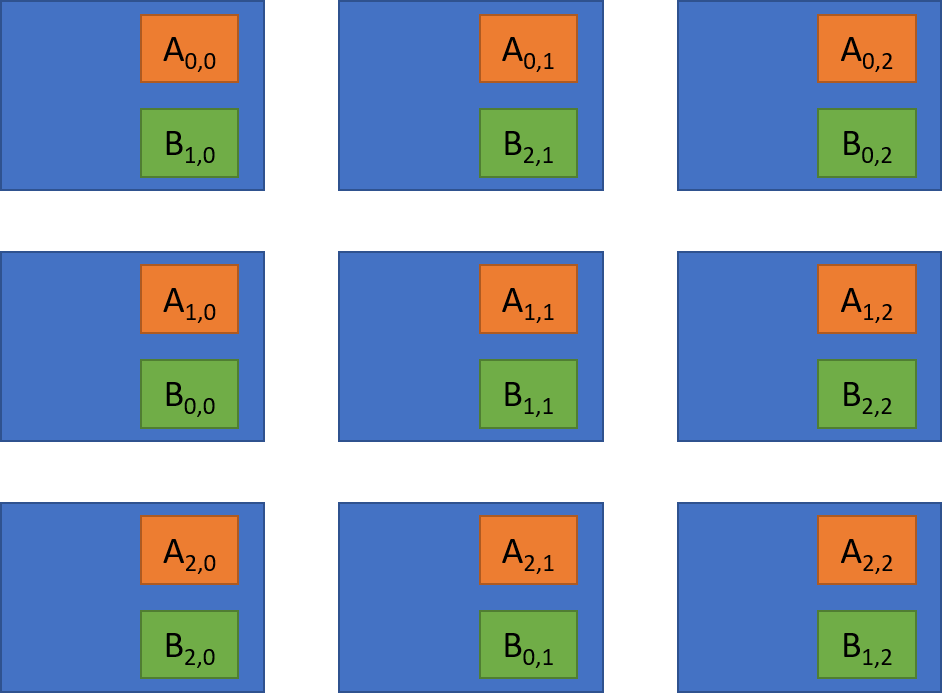
\includegraphics[width=0.72\linewidth]{figures/step_0_cannon.png}
%		\caption{Starting Point}
%	\end{figure}
%\end{frame}

\begin{frame}{Cannon's Algorithm}
	\begin{figure}	
		\centering
		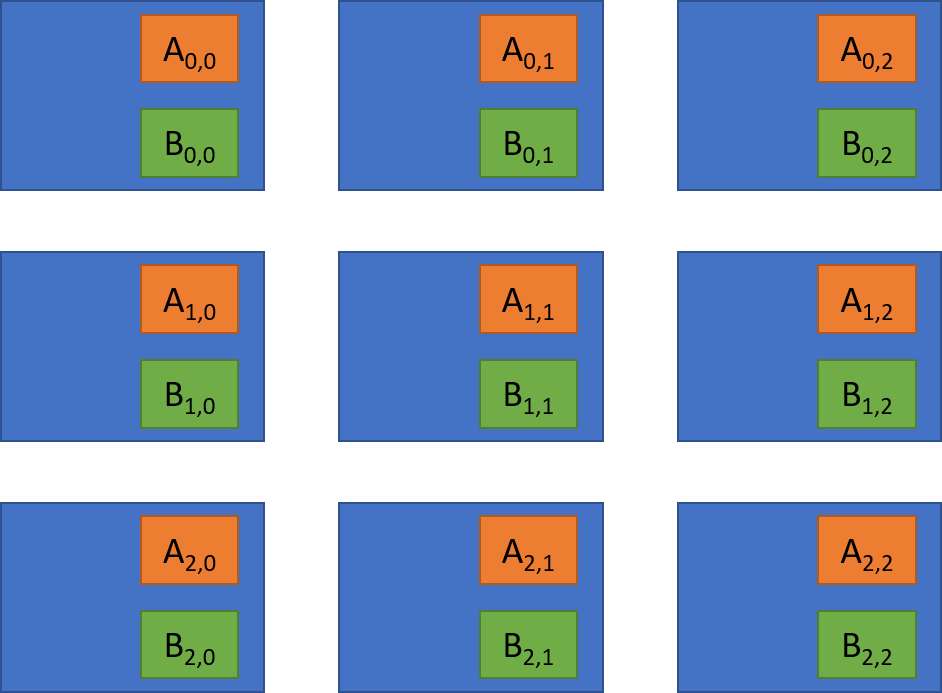
\includegraphics[width=0.72\linewidth]{figures/step_1_cannon.png}
		\caption{Alignment}
	\end{figure}
\end{frame}

\begin{frame}{Cannon's Algorithm}
	\begin{figure}	
		\centering
		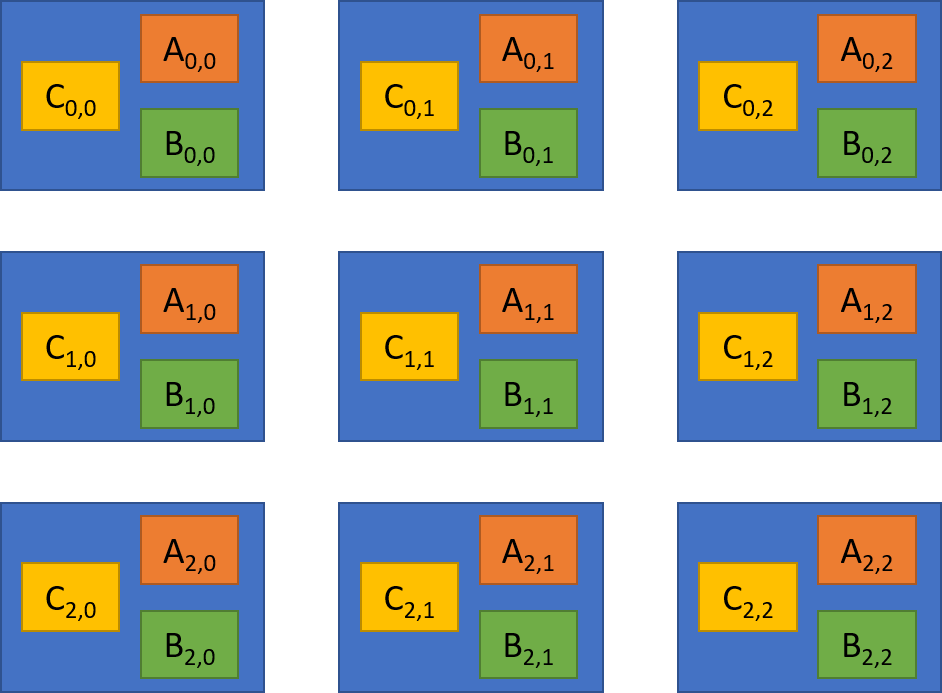
\includegraphics[width=0.72\linewidth]{figures/step_2_cannon.png}
		\caption{Multiply Local Values}
	\end{figure}
\end{frame}

\begin{frame}{Cannon's Algorithm}
	\begin{figure}	
		\centering
		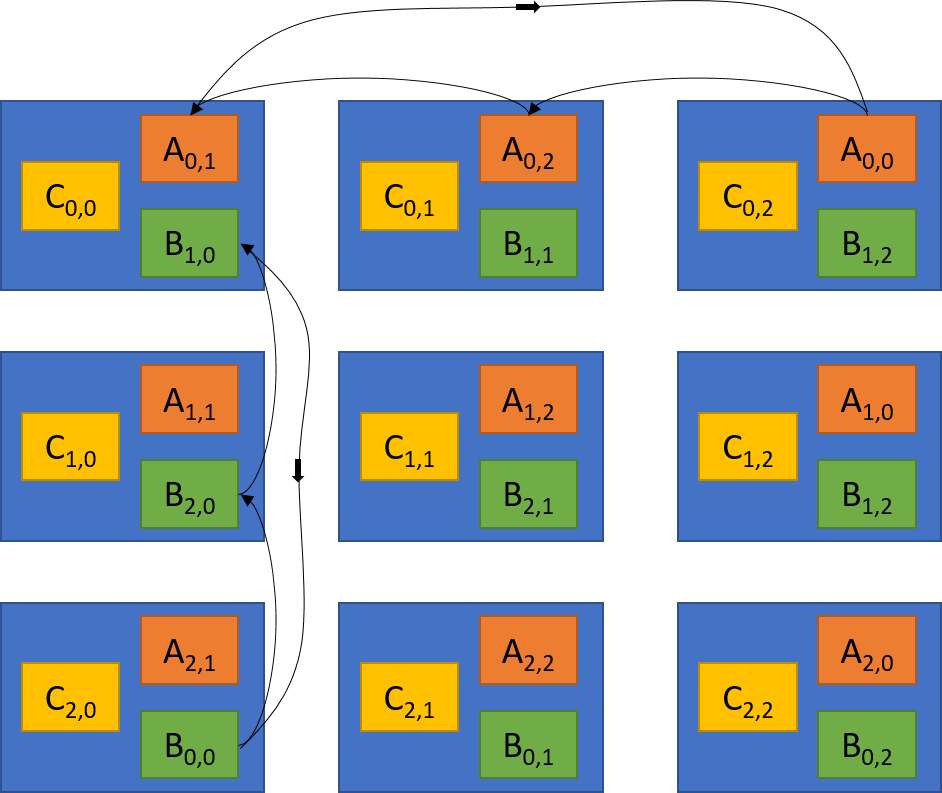
\includegraphics[width=0.72\linewidth]{figures/step_3_cannon.png}
		\caption{Shift Data \& multiply}
	\end{figure}
\end{frame}

%\begin{frame}{Cannon's Algorithm}
%\begin{figure}	
%\centering
%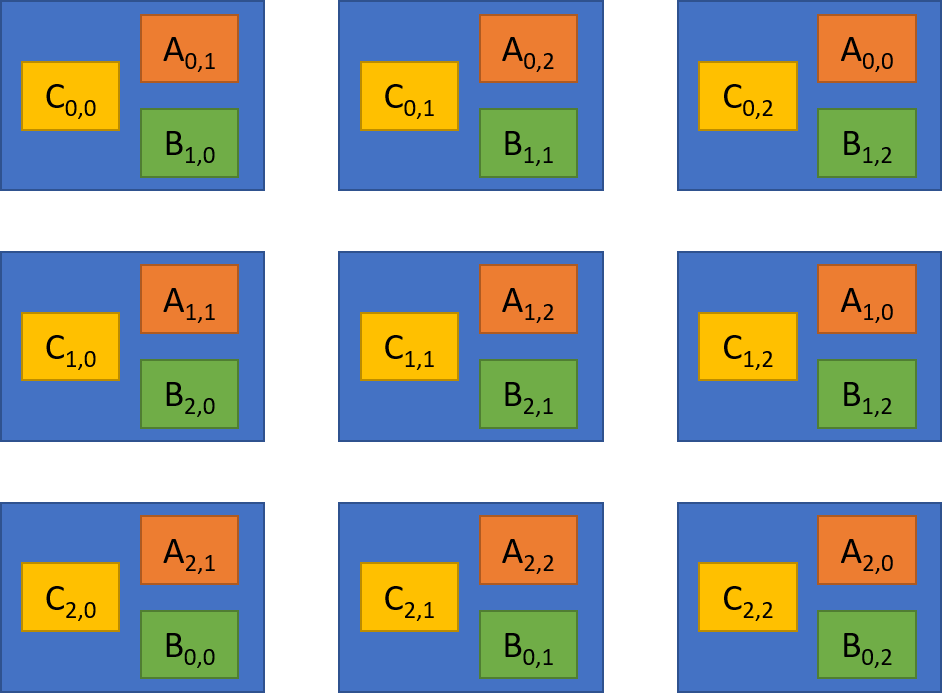
\includegraphics[width=0.72\linewidth]{figures/step_2_cannon_2.png}
%\caption{Multiply Local Values}
%\end{figure}
%\end{frame}

\begin{frame}{Cannon's Algorithm}
\begin{figure}	
	\centering
	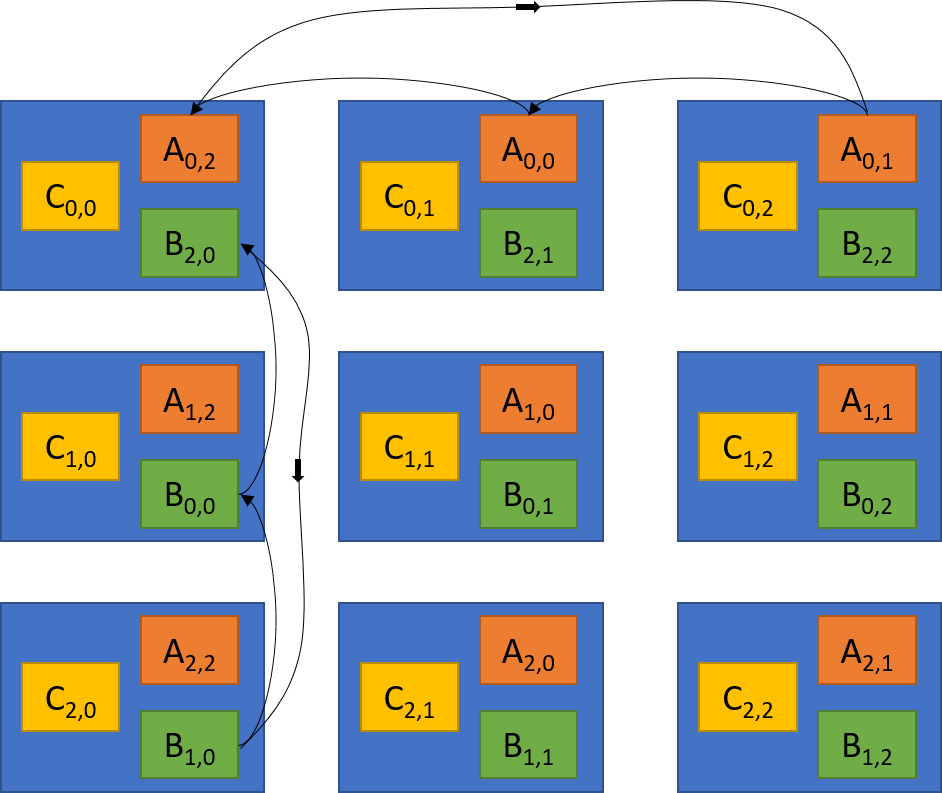
\includegraphics[width=0.72\linewidth]{figures/step_3_cannon_2.png}
	\caption{Shift Data \& multiply}
\end{figure}
\end{frame}

\begin{frame}{Cannon's Algorithm}
	\begin{figure}	
		\centering
		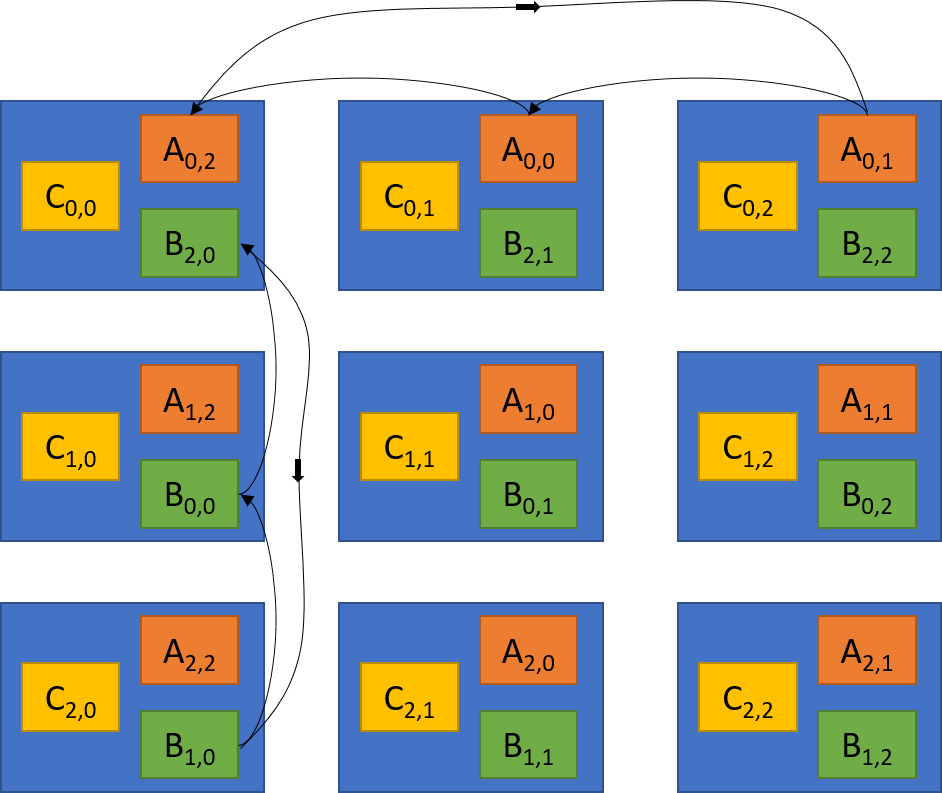
\includegraphics[width=0.72\linewidth]{figures/step_3_cannon_2.png}
		\caption{Shift Data \& multiply}
	\end{figure}
\end{frame}

\begin{frame}{Futurizing Cannon's Algorithm}
	\begin{outline}
		\1 No permanent data moving
			\2 Pulling instead
			\2 Doubles memory cost
		\1 Allows pulling to be done one cycle ahead
	\end{outline}
\end{frame}

%\begin{frame}{Cannon's Algorithm}
%\begin{figure}	
%	\centering
%	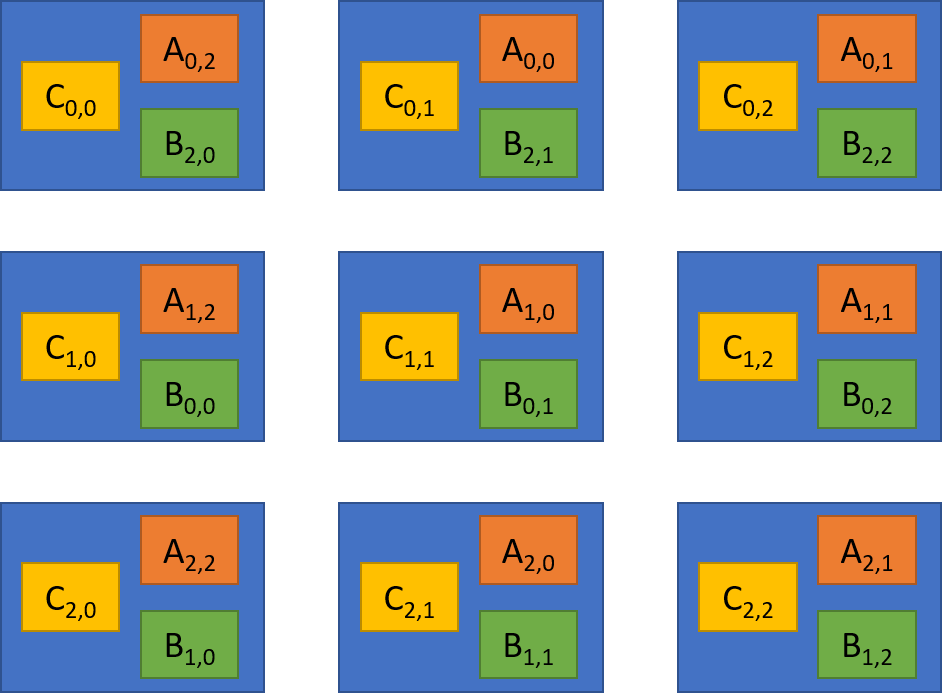
\includegraphics[width=0.72\linewidth]{figures/step_2_cannon_3.png}
%	\caption{Multiply Local Values}
%\end{figure}
%\end{frame}
\section{Results}

\begin{frame}{Preliminary Results}
	\begin{columns}
		\column{0.4\linewidth}
		\begin{outline}
			\1 Both distributed algorithms outperformed the pure serial version
			\1 Cannon performed substantially better than dot\_d
		\end{outline}

		\column{0.75\linewidth}
		\centering
		\begin{tabular}{|c|c|c|c|c|} \hline
			Matrix Size & dot\_d & cannon & dot (serial)\\ \hline
			500 & 5589.92 & 2519.04 & 8566.63 \\ \hline
			1000 & 36991.6 & 25815.2 & 67518.4 \\ \hline
			2000 & 283583 & 203211 & 538530 \\ \hline
		\end{tabular}
	\end{columns}
\end{frame}

\begin{frame}[standout]
	Questions?
\end{frame}

\end{document}
